% !Mode:: "TeX:UTF-8" 

\BiSection{2.6}{Figures}

解:

\scalebox{3}{(a)}

为确保PFET在饱和区,需要$V_{SG}>|V_{TH}|$

$(V_{DD}-V_{X})\frac{R_1}{R_1+R_2}>-V_{TH}$

$V_{X}<V_{DD}+V_{TH}(1+\frac{R_2}{R_1})$

	\color{blue}{
	\{
	
	当$V_{GS}+|V_{TH}|>V_{GS}>V_{DS}$即$V_{G}>V_{D}$时,PFET在饱和区。由电路图得栅极总是大于漏极(PFET电压低的为漏极)
	
	\begin{figure}[H] %H为当前位置,!htb为忽略美学标准,htbp为浮动图形
		\begin{minipage}{\linewidth}
			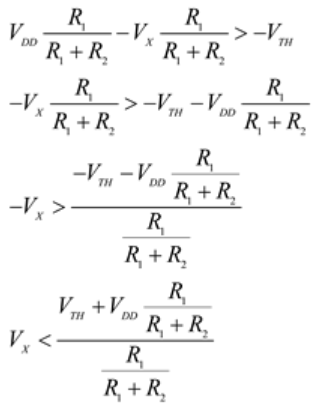
\includegraphics{2.6-1}
		\end{minipage}
	\end{figure}
	
		\begin{figure}[H] %H为当前位置,!htb为忽略美学标准,htbp为浮动图形
		\begin{minipage}{\linewidth}
			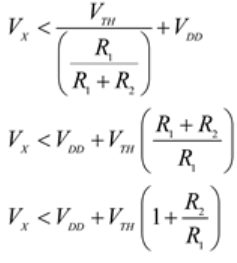
\includegraphics{2.6-2}
		\end{minipage}
	\end{figure}
	
	
	
	
	
	
	\}
	
	
	
	
	
	
}









\color{black}{

	$I_X=I_D=\frac{1}{2}\mu_pC_{ox}\frac{W}{L}[V_{SG}-(-V_{TH})]^2=\frac{1}{2}\mu_pC_{ox}\frac{W}{L}[(V_{DD}-V_{X})\frac{R_1}{R_1+R_2}-(-V_{TH})]^2$

	$g_m=\sqrt{2\mu_pC_{ox}\frac{W}{L}I_D}=\sqrt{2\mu_pC_{ox}\frac{W}{L}\{\frac{1}{2}\mu_pC_{ox}\frac{W}{L}[(V_{DD}-V_{X})\frac{R_1}{R_1+R_2}-(-V_{TH})]^2\}}=\mu_pC_{ox}\frac{W}{L}[(V_{DD}-V_{X})\frac{R_1}{R_1+R_2}-(-V_{TH})]$

		\begin{figure}[H] %H为当前位置,!htb为忽略美学标准,htbp为浮动图形
	\begin{minipage}{\linewidth}
		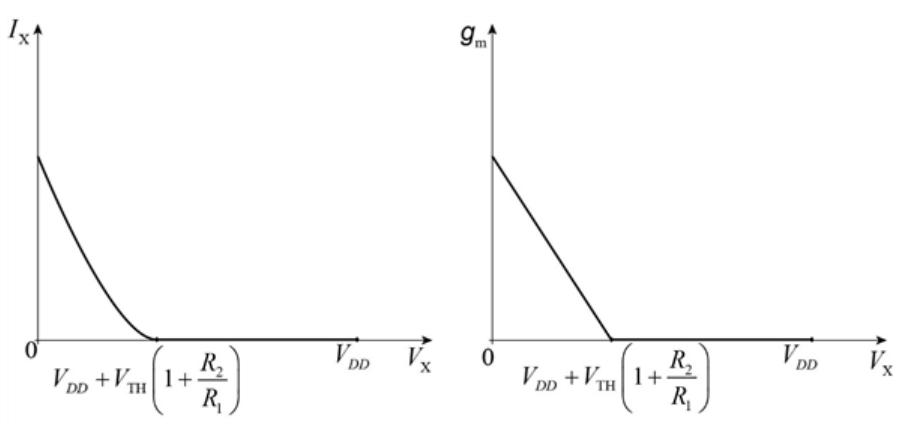
\includegraphics{2.6-3}
	\end{minipage}
	\caption*{图1} %最终文档中希望显示的图片标题
\end{figure}

\scalebox{3}{(b)}

为确保NFET在饱和区,需要$V_{GS}>V_{TH}$

$(V_{DD}-V_{X})\frac{R_2}{R_1+R_2}>V_{TH}$

$V_{X}<V_{DD}-V_{TH}(1+\frac{R_1}{R_2})$


}
\color{blue}{
	\{
	
	当$V_{GS}-V_{TH}<V_{GS}<V_{DS}$即$V_{G}<V_{D}$时,NFET在饱和区。由电路图得栅极总是小于漏极(NFET电压高的为漏极)
	
	\begin{figure}[H] %H为当前位置,!htb为忽略美学标准,htbp为浮动图形
		\begin{minipage}{\linewidth}
			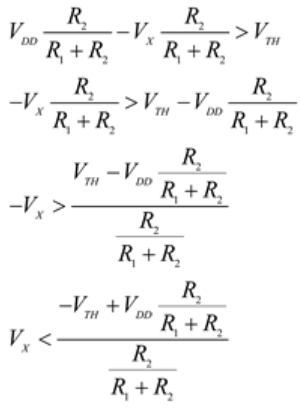
\includegraphics{2.6-4}
		\end{minipage}
	\end{figure}
	
	\begin{figure}[H] %H为当前位置,!htb为忽略美学标准,htbp为浮动图形
		\begin{minipage}{\linewidth}
			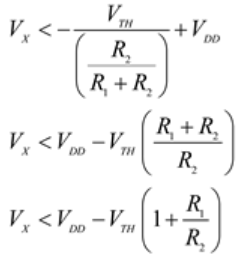
\includegraphics{2.6-5}
		\end{minipage}
	\end{figure}
	
	
	\}
	
	
	
}
\color{black}{
	
	$I_X=I_D=\frac{1}{2}\mu_nC_{ox}\frac{W}{L}(V_{GS}-V_{TH})^2=\frac{1}{2}\mu_nC_{ox}\frac{W}{L}[(V_{DD}-V_{X})\frac{R_2}{R_1+R_2}-V_{TH}]^2$
	
	$g_m=\sqrt{2\mu_nC_{ox}\frac{W}{L}I_D}=\sqrt{2\mu_nC_{ox}\frac{W}{L}\{\frac{1}{2}\mu_nC_{ox}\frac{W}{L}[(V_{DD}-V_{X})\frac{R_2}{R_1+R_2}-V_{TH}]^2\}}=\mu_nC_{ox}\frac{W}{L}[(V_{DD}-V_{X})\frac{R_2}{R_1+R_2}-V_{TH}]$
	
	\begin{figure}[H] %H为当前位置,!htb为忽略美学标准,htbp为浮动图形
		\begin{minipage}{\linewidth}
			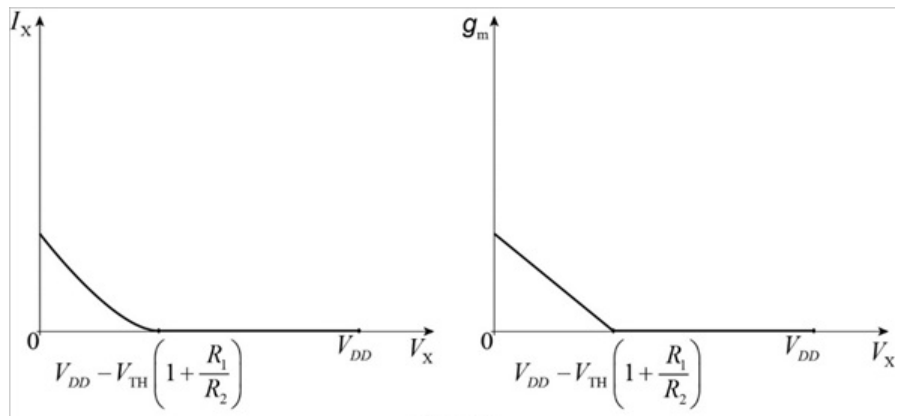
\includegraphics{2.6-6}
		\end{minipage}
		\caption*{图2} %最终文档中希望显示的图片标题
	\end{figure}
	
	\scalebox{3}{(c)}
	
	因为由电路图得电阻电流$I_{R1}=I_1-I_X$,所以$0 \leq I_X \leq I_1$
	
	$V_{GS}=2-V_X+R_1(I_1-I_X)$
	
	$V_{DS}=R_1(I_1-I_X)$
	
	当$V_{GS}-V_{TH}>V_{DS}$即$2-V_{TH}>V_{X}>0$时,NFET在线性区
	
	$I_X=I_D=\mu_nC_{ox}\frac{W}{L}[(V_{GS}-V_{TH})V_{DS}-\frac{1}{2}V_{DS}^2]=\mu_nC_{ox}\frac{W}{L}\{[2-V_X+R_1(I_1-I_X)-V_{TH}]R_1(I_1-I_X)-\frac{1}{2}[R_1(I_1-I_X)]^2\}$
	
	$g_m=\mu_nC_{ox}\frac{W}{L}V_{DS}=\mu_nC_{ox}\frac{W}{L}R_1(I_1-I_X)$
	
		当$V_{GS}<V_{TH}$即$V_{X}>2-V_{TH}+R_1I_1-R_1I_X$时,NFET关
	
	当$2-V_{TH}<V_{X}<2-V_{TH}+R_1I_1-R_1I_X$时,NFET在饱和区
	
	$I_X=I_D=\frac{1}{2}\mu_nC_{ox}\frac{W}{L}(V_{GS}-V_{TH})^2=\frac{1}{2}\mu_nC_{ox}\frac{W}{L}[2-V_X+R_1(I_1-I_X)-V_{TH}]^2$
	
	$g_m=\sqrt{2\mu_nC_{ox}\frac{W}{L}I_D}=\sqrt{2\mu_nC_{ox}\frac{W}{L}\{\frac{1}{2}\mu_nC_{ox}\frac{W}{L}[2-V_X+R_1(I_1-I_X)-V_{TH}]^2\}}=\mu_nC_{ox}\frac{W}{L}[2-V_X+R_1(I_1-I_X)-V_{TH}]$
	

	
		\begin{figure}[H] %H为当前位置,!htb为忽略美学标准,htbp为浮动图形
		\begin{minipage}{\linewidth}
			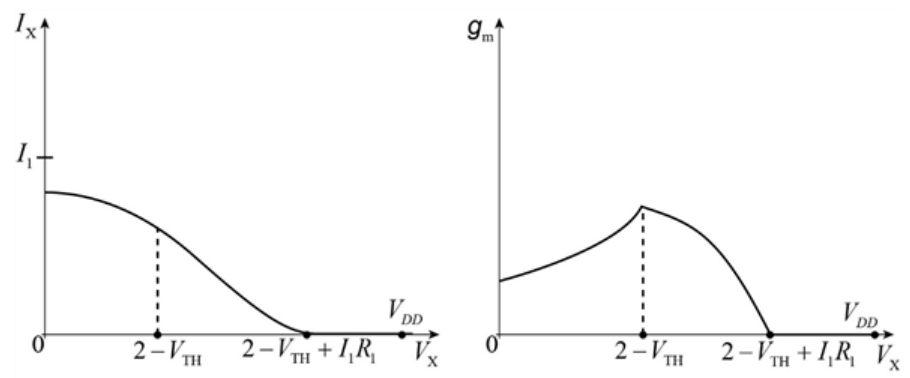
\includegraphics{2.6-7}
		\end{minipage}
		\caption*{图3} %最终文档中希望显示的图片标题
	\end{figure}
	
		\scalebox{3}{(d)}
	
		$V_{GS}=R_1(I_1-I_X)$
	
		$V_{DS}=2-V_{X}+R_1(I_1-I_X)$
		
		因为当$V_{GS}<V_{TH}$即$V_{TH}>R_1(I_1-I_X)$时,NFET关,所以假设$R_1(I_1-I_X)$大于阈值电压
	
		当$V_{GS}-V_{TH}<V_{DS}$即$2+V_{TH}>V_{X}>0$时,NFET在饱和区
	
	$I_X=I_D=\frac{1}{2}\mu_nC_{ox}\frac{W}{L}(V_{GS}-V_{TH})^2=\frac{1}{2}\mu_nC_{ox}\frac{W}{L}[R_1(I_1-I_X)-V_{TH}]^2$
	
	$g_m=\sqrt{2\mu_nC_{ox}\frac{W}{L}I_D}=\sqrt{2\mu_nC_{ox}\frac{W}{L}\{\frac{1}{2}\mu_nC_{ox}\frac{W}{L}[R_1(I_1-I_X)-V_{TH}]^2\}}=\mu_nC_{ox}\frac{W}{L}[R_1(I_1-I_X)-V_{TH}]$
	
	当$2+V_{TH}<V_{X}$时,NFET在线性区
	
	$I_X=I_D=\mu_nC_{ox}\frac{W}{L}[(V_{GS}-V_{TH})V_{DS}-\frac{1}{2}V_{DS}^2]$
	
			\begin{figure}[H] %H为当前位置,!htb为忽略美学标准,htbp为浮动图形
		\begin{minipage}{\linewidth}
			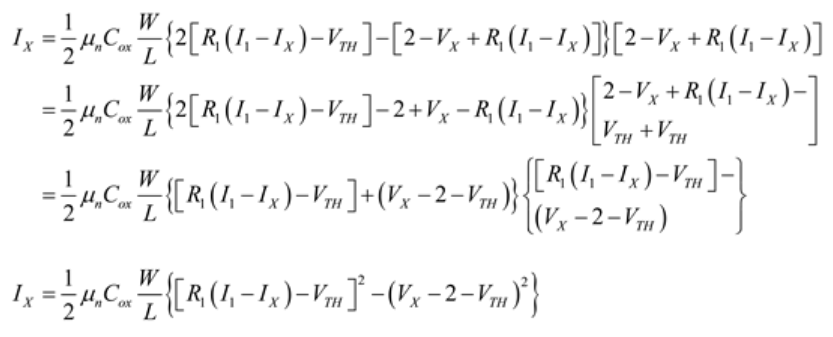
\includegraphics{2.6-8}
		\end{minipage}
	\end{figure}
	
	上式表示电流随着电压的增加而减小。因此,电流的极性随着电压的增加而变化。
	
		$g_m=\mu_nC_{ox}\frac{W}{L}V_{DS}=\mu_nC_{ox}\frac{W}{L}[2-V_{X}+R_1(I_1-I_X)]$
	
			\begin{figure}[H] %H为当前位置,!htb为忽略美学标准,htbp为浮动图形
		\begin{minipage}{\linewidth}
			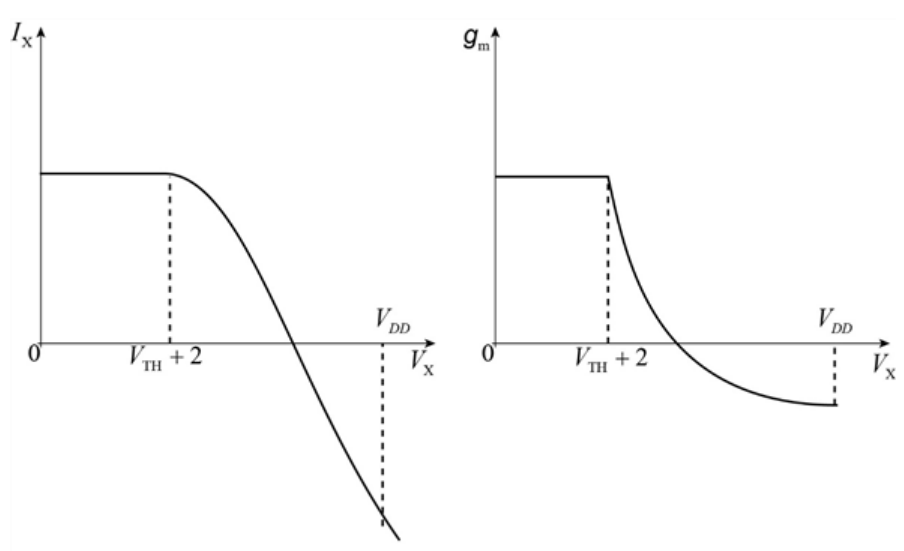
\includegraphics{2.6-9}
		\end{minipage}
		\caption*{图4} %最终文档中希望显示的图片标题
	\end{figure}
	
			\scalebox{3}{(e)}
	
	当$V_{TH}>V_{X}>0$时,NFET关
	
	$V_{GS}=V_{X}$
	
	$V_{DS}=V_{X}-R_1(I_X-I_1)$
	
	当NFET在饱和区时,$V_{GS}-V_{TH}<V_{DS}$即$\sqrt{\frac{2I_1+\frac{2V_{TH}}{R_1}}{\mu_nC_{ox}\frac{W}{L}}}+V_{TH}>V_{X}>V_{TH}$
	
}

\color{blue}{
	
\{

令$V_{GS}-V_{TH}=V_{DS}$

$V_{X}-V_{TH}=V_{X}-R_1(I_X-I_1)$

$V_{TH}=R_1(I_X-I_1)$

			\begin{figure}[H] %H为当前位置,!htb为忽略美学标准,htbp为浮动图形
	\begin{minipage}{\linewidth}
		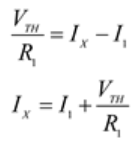
\includegraphics{2.6-10}
	\end{minipage}
\end{figure}

			\begin{figure}[H] %H为当前位置,!htb为忽略美学标准,htbp为浮动图形
	\begin{minipage}{\linewidth}
		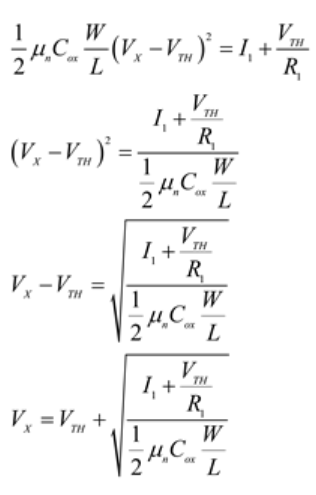
\includegraphics{2.6-11}
	\end{minipage}
\end{figure}

$\sqrt{\frac{2I_1+\frac{2V_{TH}}{R_1}}{\mu_nC_{ox}\frac{W}{L}}}+V_{TH}=V_{X}$

\}

}

\color{black}{
	
	$I_X=\frac{1}{2}\mu_nC_{ox}\frac{W}{L}(V_{X}-V_{TH})^2$
	
	$g_m=\sqrt{2\mu_nC_{ox}\frac{W}{L}\{\frac{1}{2}\mu_nC_{ox}\frac{W}{L}(V_{X}-V_{TH})^2\}}=\mu_nC_{ox}\frac{W}{L}(V_{X}-V_{TH})$
	
	当$\sqrt{\frac{2I_1+\frac{2V_{TH}}{R_1}}{\mu_nC_{ox}\frac{W}{L}}}+V_{TH}<V_{X}$时,NFET在线性区
	
	$I_X=I_D=\mu_nC_{ox}\frac{W}{L}[(V_{GS}-V_{TH})V_{DS}-\frac{1}{2}V_{DS}^2]=\mu_nC_{ox}\frac{W}{L}\{(V_{X}-V_{TH})[V_{X}-R_1(I_X-I_1)]-\frac{1}{2}[V_{X}-R_1(I_X-I_1)]^2\}$
	
				\begin{figure}[H] %H为当前位置,!htb为忽略美学标准,htbp为浮动图形
		\begin{minipage}{\linewidth}
			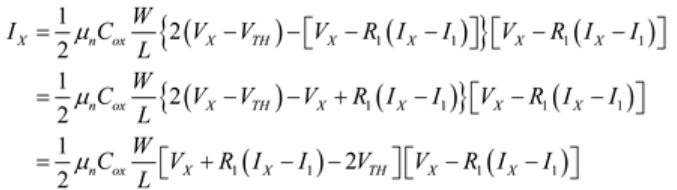
\includegraphics{2.6-13}
		\end{minipage}
	\end{figure}
	
	$g_m=\mu_nC_{ox}\frac{W}{L}V_{DS}=\mu_nC_{ox}\frac{W}{L}[V_{X}-R_1(I_X-I_1)]$
	
	
	
	

			\begin{figure}[H] %H为当前位置,!htb为忽略美学标准,htbp为浮动图形
	\begin{minipage}{\linewidth}
		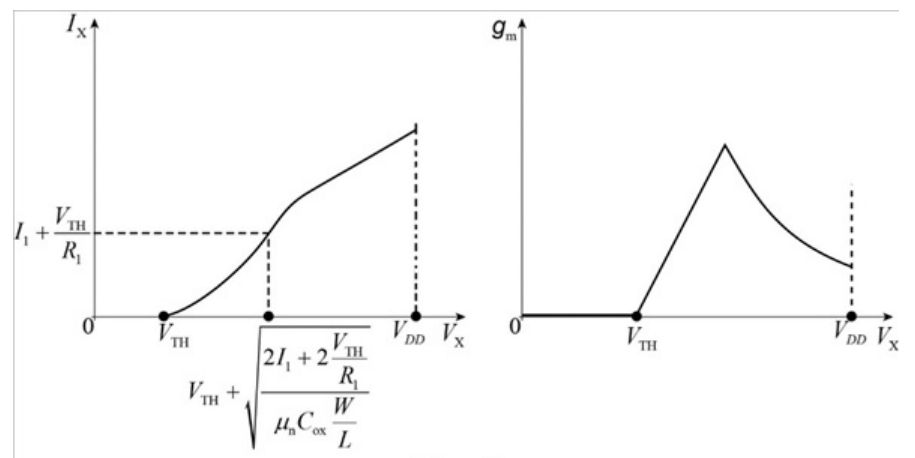
\includegraphics{2.6-12}
	\end{minipage}
	\caption*{图5} %最终文档中希望显示的图片标题
\end{figure}

}

	\color{green}{
		
	\{
	
	
	\ding{172}(c)和(d)中NFET关的$-R_1I_X$与英文答案不同和……
	
	\ding{173}(d)线性区分析电流公式
	
	
	
	
	
	
	\}
	
	
	
	
	
	
}









\color{black}{

}

